\documentclass[twocolumn, 10pt]{article}
\usepackage{graphicx}
\usepackage{hyperref}
\usepackage{amsmath}
\usepackage{float}
\usepackage{enumitem}
\usepackage{listings}
\usepackage{todonotes}
\newcommand{\varA}[1]{{\operatorname{#1}}}
\setlength{\marginparwidth}{2cm} %necessary for todonotes to work on left margin

\begin{document}
\title{Graphische Programmierung der klassischen Mechanik}
\author{github.com/kloimhardt}
\maketitle

\renewcommand{\abstractname}{Abstract}
\abstract
In the presentation of Classical Mechanics at university level, Computer Algebra Systems\todo{Not everyone knows what a CAS is} are used since years. The further dissemination of interactive computer work in physics classes seems desirable. To this end, graphical interfaces which allow the student to seamlessly switch into a professional development environment could be introduced. In this article, we present an interface which allows to conduct computer experiments of Classical Mechanics. The syntax of the thereby used functional programming paradigm leads itself perfectly to an implementation as graphical blocks. The system is designed for interactive classroom lectures. Upon suitable preparation, only the computer mouse, i.e. no keyboard, is needed during the lecture. The lecturer therefore does not necessarily need to have any programming experience. However, a realworld test of the system is pending. Moreover, the execution of the programs is deliberately denoted as conducting an experiment. The interactive work with the graphical blocks is meant to evoke a change to this perspective.

\renewcommand{\abstractname}{Kurzfassung}
\abstract
In der Hochschuldidaktik der klassischen Mechanik werden Computeralgebrasysteme (CAS) schon seit Jahren eingesetzt. Die weitere Verbreitung der interaktiven Computerarbeit im Physikstudium scheint\todo{ist oder ist nicht; Ausdruck scheint wage} wünschenswert. Dafür können anfängerfreundliche graphische Oberflächen dienen, die es dem Studierenden ermöglichen, nahtlos in eine professionelle Entwicklungsumgebung zu wechseln. In diesem Artikel wird eine Oberfläche vorgestellt mit welcher Computerexperimente zur klassischen Mechanik durchgeführt werden können. Diese basiert auf dem sogenannten funktionalen Programmieransatz, dessen Syntax für eine Umsetzung in graphische Blöcke wie geschaffen\todo{Stil: besonders geeignet} ist. Die Oberfläche ist für interaktive Vorträge\todo{Nur für den Vortrag geeignet? Nein, auch zum Modellieren! Willst du das dafür empfehlen? Erklären!} direkt im Hörsaal konzipiert. Bei entsprechender Vorbereitung wird während des Vortrags nur die Computermaus, d.h. also keine Tastatur, benötigt\todo{Hölzern. Fachausdruck Drag and Drop? Physische Tastatur nie nötig, kann eingeblendet werden. Verbessern!}. Der Vortragende braucht daher nicht zwingend über Programmiererfahrung zu verfügen. Ein Praxistest des Systems im Hörsaal steht jedoch aus. Weiters wird in diesem Artikel das Laufenlassen\todo{Laufen- lassen kein guter Ausdruck} der Programme bewusst als Durchführung eines Experiments bezeichnet. Das interaktive Arbeiten mit den graphischen Bausteinen soll einen Wechsel zu dieser Ansicht hervorrufen.



\section{Einleitung}
In der Hochschuldidaktik der klassischen Mechanik werden Computeralgebrasysteme (CAS) und symbolisches Programmieren schon seit Jahren eingesetzt. Die bekanntesten Systeme sind Maple \cite{cSpencer 1}, Maxima \cite{cTimber 2} und vor allem Mathematica \cite{cRobi 3}. Basierend auf letztgenanntem kommt \cite{cBerta 4} zum Schluss\todo{da darauf eingegangen: Bertacchini et.al. angeben}, dass es im Moment keine effektivere Methode gibt, um die beobachteten positiven Lernerfolge zu erzielen\footnote{"today there are no other equally effective, powerful and easily adoptable tools, that allow to achieve results like those obtained"}. Nicht zuletzt aufgrund solcher Erfahrungen scheint die weitere Verbreitung der interaktiven Computerarbeit im Physikstudium wünschenswert \cite{cCaballero 5}\footnote{"few report using computation with interactive engagement methods in the classroom"}.

In dem für das Weitere grundlegenden Artikel \cite{cSussmanPaper 6} wird von Sussman et. al. gezeigt, dass bei der traditionellen Vermittlung physikalischer Theorien die Verwendung mathematischer Symbole\todo{Was ist mit Symbolen geimeint? + -? Erklären!} stark vom Kontext abhängt. Dieses Problem wird prinzipiell innerhalb aller CAS gelöst, da die Programme vom Computer interpretierbar und daher eindeutig formuliert sein müssen. Der Programmieransatz des in \cite{cSussmanPaper 6} vorgestellten SICM\todo{SICM beduetet Structure and Interpretation of Classical Mechanics} Systems erlaubt es jedoch, die Computersyntax isomorph\todo{Ausdruck unpassend und falsch, isomorph hat eine andere exakte Bedeutung} zur mathematischen Notation des zugehörigen Lehrbuchs \cite{cSICM 7} zu halten.

Ein Überblick über die generelle methodische und erkenntnistheoretische Bedeutung von Computersimulationen im Wissenschaftsunterricht findet sich in \cite{cDevelaki 8}. Bart et. al. \cite{cBartPos 9} stellen die Frage, wie Computer speziell in Hochschulstudiengängen eingeführt werden können\footnote{"How do we bring introductory computing to mature, domain-identified undergraduates, who have concerns for both their own self-efficacy and for the value in learning computing?"}. Als Antwort stellen sie eine anfängerfreundliche graphische Oberfläche vor, BlockPy, aus der die Studierenden nahtlos in eine professionelle Entwicklungsumgebung wechseln können.

Graphische Werkzeuge werden naturgemäß speziell zur Einführung in die Informatik eingesetzt, beispielsweise in \cite{cModrow 10} und \cite{cPrice 11}, wobei das Zielpublikum dieser Initiativen weit gestreut ist. Einige Untersuchungen zur Auswirkung von graphischen Programmierumgebungen auf das konzeptionelle Verständnis von Schülern werden in \cite{cXu 12} überblicksmäßig dargestellt.

Wir widersprechen mit \cite{cConversy 13}\todo{Da direkt darauf eingegangen: "... mit Conversy et. al.", widersprechen ohne Argument geht nicht} einer etwaigen Ansicht, dass visuelle Sprachen prinzipiell besser wären als textuelle. Graphische Oberflächen eignen sich aber gut für Demonstrationen, bei denen eine spezifische Thematik am Computer modelliert wird.

In diesem Artikel wird eine graphische Oberfläche vorgestellt, mittels welcher Computerexperimente\todo{Referenz zum Begriff Computerexperiment angeben} zur klassischen Mechanik durchgeführt werden können. Diese basiert auf dem oben erwähnten SICM System, dessen Syntax für eine isomorphe Abbildung in graphische Blöcke wie geschaffen\todo{besser: besonders geeignet} ist. Da einfache Lehrvideos von den Studierenden nur bedingt angenommen werden \cite{cLin 14}\footnote{"The trend of students not accessing long videos completely was more prominent in lecture-oriented videos than the laboratory videos."}, ist die Oberfläche für interaktive Vorträge direkt im Hörsaal konzipiert. Ein Praxistest des Systems im Hörsaal steht jedoch aus.\todo{Gut: zentrale Botschaft im letzten Absatz der Einleitung. Aber ein guter Überblick des Papers fehlt doch}

Weiters wird in diesem Artikel das Laufenlassen der Programme bewusst als Ausführung eines Experiments bezeichnet. Die erkenntnistheoretische Bedeutung von realen Laborexperimenten wird von Krause \cite{cKrause 15} aus dem Blickwinkel der Physikdidaktik beleuchtet. Das Erstellen von Computermodellen speziell mittels graphischer Oberfläche wird im letzten Abschnitt an diesen Begriffsrahmen angegliedert.

\section{Methoden}
Die oben genannte Bibliothek SICM ist und wird in der Sprache Scheme \cite{cScheme 16} programmiert, einem Dialekt der Programmiersprache LISP \cite{cMcCarthy 17}. Das hier vorgestellte System basiert auf einer Version der SICM Bibliothek, die in einem jüngeren LISP Dialekt implementiert wurde \cite{cColin 18}.

Alle diese Dialekte folgen dem sogenannten funktionalen Ansatz\todo{Um- formulieren, Präzisieren}, es stehen also Funktionen im Mittelpunkt. Im Gegensatz dazu wird in allen anderen vorgestellten CAS diese zentrale Stellung von sogenannten Ausdrücken, engl. Expressions\footnote{Maple Lab Manual: "Expressions are easy to plot, differentiate (with diff), or integrate, and the result is always another expression, […] the result of applying a Maple command to a function is not always a function. […] The main difference is that it is very easy to find the value of a function at a specific point or compose two functions, whereas either of these tasks for an expression involves the use of the subs command." \url{www.math.wpi.edu/Course_Materials/Maple/manual2e/node24.html}}\todo{Begriff "main difference" der Fussnote in Haupttext geben und Vorteil des funkt. Ansatz mehr herausarbeiten}, eingenommen. Der Vorteil gegenüber diesen Ausdrücken ist, dass Funktionen einfacher zu kombinieren sind, weswegen sie sich auch ideal zur Darstellung als graphische Bausteine eignen.  Ein\todo{Funktionale Programmierung bedingt Präfix Notation im Allgemeinen gar nicht; Satz woanders hin} Grund, warum der strikt funktionale Ansatz im Allgemeinen nicht verfolgt wird, ist vielleicht, dass die resultierende kompakte Syntax als schwer lesbar empfunden wird. Konkret werden oft  Präfixnotation\footnote{Die Infixnotation $5*t+2$ wird in Präfixnotation als \\ (+ (* 5 t) 2) angeschrieben.} und viele verschachtelte Klammern\footnote{Im Jargon: LISP = Lost In Stupid Parentheses, \url{en.wikipedia.org/wiki/Lisp_(programming_language)}} genannt.

Die graphische Oberfläche basiert auf Blockly \cite{cFraser 19}, sie wird im WebBrowser dargestellt. Blockly erlaubt das Auswählen, Verschieben, Herauslösen oder Löschen von graphischen Bausteinen, sogenannten Kacheln\todo{Verwende durchgehen den Begriff "Blöcke"}. Aus dem von Blockly erzeugten Datenstrukturen wird auf Knopfdruck ein LISP Programm erzeugt. Als konzeptionelles Vorbild diente das bereits oben genannte Programmpaket \todo{Ist Blockly und BlockPy dasselbe? Nein, BlockPy basiert auf Blockly!} BlockPy \cite{cBartStudy 20}, welches Python-Code erzeugt und für Datenanalysen konzipiert ist.

Ein erster Vorteil der Darstellung von Code mittels Kacheln ist die Abwesenheit der oben negativ erwähnten Klammern, die Kacheln sind auch bei komplexer Verschachtelung gut sichtbar voneinander getrennt. Dazu tragen die verschiedenen Kachelfarben bei, welche durch die Anzahl der jeweiligen Unterkacheln festgelegt sind. Die Präfixnotation wird beibehalten, um eine 1:1 Relation zwischen den Kacheln und dem Programmcode zu wahren. Algebraische Ergebnisse werden aber in gewohnter\todo{um- formulieren} Infixnotation angezeigt.

Aus eigener Erfahrung ist zum Modellieren per se die übliche textuelle Programmierweise vorzuziehen, die Oberfläche ist zur Erklärung und Variation vorbereiteter Modelle konzipiert. Bei entsprechender Vorbereitung, die nicht zwingend vom Vortragenden selbst erfolgen muss, wird während des Vortrags nur die Computermaus, d.h. also keine Tastatur, benötigt. Der Vortragende braucht daher nicht zwingend über Programmiererfahrung\todo{wirklich keine Erfahrung nötig? Erklären!} zu verfügen.

\section{Aufbau eines Computerexperiments}\todo{Titel sehr gewagt und miss- verständlich}

Die Bewegungsgleichung des freien Teilchens lautet in üblicher Schreibweise:

\begin{equation}
m \frac{\mathrm d^2 \vec{x}}{\mathrm d t^2}=0
\label{eq:newton}
\end{equation}

Dabei stellt m die Masse und der Vektor $ \vec{x}$ die Ortskoordinaten des Teilchens dar. Die zweite Ableitung des Ortes nach der Zeit ist seine Beschleunigung. Ein Massenpunkt im leeren kräftefreien Raum ändert seine Geschwindigkeit niemals, denn nichts ruft eine Beschleunigung hervor, welche daher den Wert Null annimmt.

Die Gleichung soll nun mit der SICM Bibliothek für zwei Raumdimensionen zuerst generiert\todo{Was heisst generiert? Was ist der Sinn der Übung? Erklären!} und dann eingehend untersucht werden. Dazu werden mittels der graphischen Oberfläche als erstes folgende zwei Funktionen definiert:
\begin{enumerate}[label=(\alph*)]
\item $\varA{Path-of-a-Free-Particle(time)}$: Pfad eines freien Teilchens in zwei Dimensionen.\todo{Ist das ein Beispielpfad? Ja!}

\begin{equation}
\vec{x} = \begin{pmatrix} x(t) \\ y(t) \end{pmatrix} =
\begin{pmatrix}5t + 2 \\ 4t + 3\end{pmatrix}
\end{equation}

\item $\varA{Kinetic-Energy(velocity)}$: Kinetische Energie, vorerst einfach als das
  Quadrat der Geschwindigkeit, also für den Fall $m=2$\todo{m=2 kg, t=10 sec}.

\begin{equation}
K(\vec{v}) = \vec{v}^2
\end{equation}
\end{enumerate}

\begin{figure}[h]
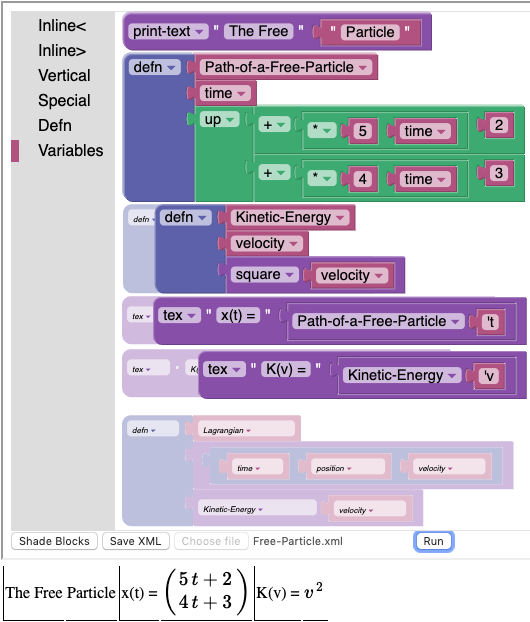
\includegraphics[scale=0.4]{bilder/session_11.png}
\caption{Die Definition des Beispielpfades und der kinetischen Energie mittels der graphischen Bausteine (Kacheln). Durch drücken auf den "Run" Button werden die entsprechenden Ausdrücke am unteren Rand sichtbar.}
\label{fig:session11}
\end{figure}

Abb. \ref{fig:session11} zeigt\todo{Abb nicht nachvollziehbar. Ist das am unteren Rand das Ergebnis? Ja, mit dem Begriff "Ergebnis" ist der TeX Ausdruck gemeint!} die Definition der Funktionen in der Oberfläche. Die am linken Rand teilweise sichtbaren Schattenblöcke und vor allem der letzte Schattenblock sind inaktiv. So können vorbereitete Blockgruppen als Vorlage geladen werden, um sie dann durch interaktive Nachbildung zu erklären. Dazu werden die Kacheln mittels der Menüpunkte links ausgewählt (Abb. \ref{fig:session21}). 
\begin{figure}[H]
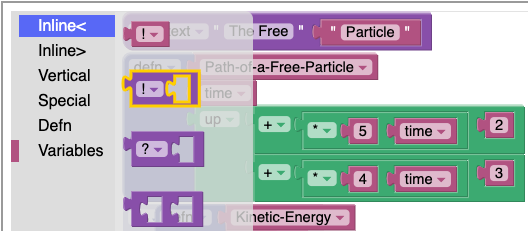
\includegraphics[scale=0.4]{bilder/session_21.png}
\caption{Auswahl einer Kachel über das Menü.}
\label{fig:session21}
\end{figure}

Die Variablen und Funktionsnamen wurden zum besseren Verständnis voll ausgeschrieben. Gewöhnungsbedürftig wird sein, dass wegen der erwähnten Präfixnotation etwa das Multiplikationszeichen * wie jede andere Funktion ganz links in der Kachel steht\todo{nicht ausreichend beschrieben}. Die letzten beiden aktiven Blöcke sorgen für die Darstellung der Funktionen als Ausdrücke in üblicher Infixnotation\todo{klingt wie ein Widerspruch}, welche am unteren Rand zu sehen ist.

Im folgenden Unterabschnitt wird erklärt, wie aus der kinetischen Energie eine Funktion "Free-Motion“ abgeleitet wird, welche die Bewegungsgleichung \ref{eq:newton} in einem danach noch zu erforschenden Sinne repräsentiert. Der Vorteil eines Computerexperiments ist aber gerade, dass die Theorie dem Studierenden nur für die verwendeten Teile bekannt sein muss. Der erstmalige Leser sollte daher nun zum nächsten Abschnitt, "Laufenlassen der Computerexperimente“, springen.

\subsection{Setup der Bewegungsgleichung}
Die Herleitung von \ref{eq:newton} aus der kinetischen Energie erfolgt mittels des Formalismus der Lagrange Mechanik.

\subsubsection{Die Lagrangefunktion}

ist in Abb. \ref{fig:session11} als Schattenblock sichtbar. Sie ist im Grunde einfach die kinetische Energie, hat aber aus technischen Gründen drei Argumente:
\begin{enumerate}[label=(\alph*)]
\setcounter{enumi}{2}
\item $\varA{Lagrangian(time, position, velocity)}$: Lagrangefunktion des freien Teilchens.
\begin{equation}
L(t, \vec{x}, \vec{v}) = K(\vec{v})
\end{equation}
\end{enumerate}

Der nächste Unterabschnitt ist ohne Kenntnis der in \cite{cSICM 7} dargestellten Theorie nicht komplett verständlich. Beispielsweise kommt erstmalig das Konzept vor, dass eine Funktion eine andere Funktion als Argument besitzt und in einer neuen Funktion resultiert. Jedoch ist die dadurch notwendig werdende Verschachtelung der Kacheln rein durch eine Betrachtung der Abbildungen beschreibbar. Diese wird gleich nach den nächsten 20 schwierigen Zeilen, im darauffolgenden Unterabschnitt, vorgenommen

\subsubsection{Die Bewegungsgleichung}

wird im Körper der folgenden Funktion erzeugt:

\begin{enumerate}[label=(\alph*)]
\setcounter{enumi}{3}
\item $\varA{Free-Motion(path-function, time)}$
\end{enumerate}

\begin{figure}[H]
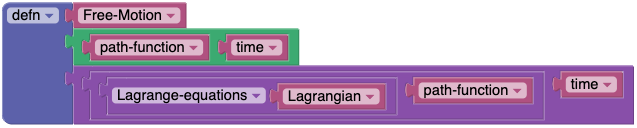
\includegraphics[scale=0.35]{bilder/session_31.png}
\caption{Konstruktion und Anwendung der Lagran-ge’schen Differentialgleichung zur Erzeugung der Bewegungsgleichung \ref{eq:newton}. }
\label{fig:session31}
\end{figure}

Dabei passiert in diesem letzten Block folgendes:

\begin{enumerate}[label=(\alph*)]
\item Konstruktion der Lagrange'schen Differential-gleichungen (LDgl) aus der Lagrangefunktion. In LISP-Syntax lautet der Befehl: 
$\varA{(Lagrange-equations \ Lagrangian)}$
\item Anwendung der LDgl auf den Pfad. Durch symbolische Differentiation erfolgt dabei beispielsweise die Ermittlung der zeitabhängigen Geschwindigkeit des Pfades. Der gesamte Vorgang resultiert in einer neuen Funktion, welche proportional der zweimalig nach der Zeit abgeleiteten path-function ist.
\item Auswertung dieser Funktion für jenen Zeitpunkt, der durch das Argument time, einer beliebigen Zahl, gegeben ist.
\end{enumerate}

\subsubsection{Die tiefste Ebene der Verschachtelung}
kommt, bei Betrachtung des letzten Blockes von Abb. \ref{fig:session31}, an genau der ersten Stelle jeder Kachel vor. Anders gesagt: beim Vergleich dieses Blocks mit allen vorhergehenden Blöcken fällt auf, dass die Sache von links her verwickelt beginnt und nach rechts gehend immer einfacher wird. Im Gegensatz dazu nimmt in allen vorhergehenden Blöcken von links einfach beginnend die Verschachtelung nach rechts gehend zu. Diese Blöcke bergen also eine aus der Schulalgebra bekannte baumartige Verzweigung. Jene unnatürliche Art der Verschachtelung im letzten Block repräsentiert das Kernkonzept des funktionalen Ansatzes und ist dessen wesentlicher Vorteil bei der Darstellung der Theorie. Die Oberfläche trägt hilfreich zum Verständnis bei, da durch Rahmung und vertikale Versetzung der Kacheln die Abgrenzung der Programmfunktionen ganz gut ersichtlich wird.

Zum selbständigen Arbeiten mit den Modellen wird auch der Studierende\todo{Gendern! Gendern!} ab einem gewissen Zeitpunkt auf den generierten Programmtext zugreifen, dieser sollte dafür auf jeden Fall manuell formatiert werden. Hauptsächlich wird dies durch horizontale Versetzung der Klammerausdrücke geschehen, sodass der obige Block wie folgt aussehen wird\footnote{Siehe speziell die entsprechenden Abb.17 und Abb.18 in \cite{cConversy 13}.}:

\begin{lstlisting}
(((Lagrange-equations Lagrangian)
     path-function)
       time)
\end{lstlisting}

\subsection{3.2.	Laufenlassen der Computerexperimente}

\todo{Was ist eigentlich das Ergebnis dieses "Experiments"? Ist auch ein Ergebnis dass die Beschleunigung zur Zeit 10 gleich 0 ist? Das Ergebnis ist der TeX Ausdruck am unteren Rand!}Die Funktion ''Free-Motion'' repräsentiert die Bewegungsgleichung \ref{eq:newton} für das freie Teilchen mit Masse m=2. Sie hat zwei Argumente: eine Pfadfunktion und einen Zeitpunkt, der sogleich als 10 festgelegt werden soll. Der Aufruf sieht folgendermaßen aus:

\begin{figure}[H]
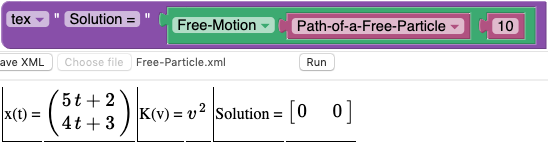
\includegraphics[scale=0.4]{bilder/session_41.png}
\caption{Die Lösung der Bewegungsgleichung \ref{eq:newton} für unseren Beispielpfad ist der Nullvektor.}
\label{fig:session41}
\end{figure}

Das Ergebnis ist der Nullvektor. Dies ist nicht verwunderlich, denn die Funktion ''Path-of-a-Free-Particle'' stellt ihrerseits einen physikalisch richtigen Pfad des freien Teilchens dar. Die Studierende wird leicht herausfinden, dass dieses Ergebnis auch dann unverändert bleibt, wenn sie einen beliebigen anderen Zeitpunkt oder andere Werte\todo{Was heisst Werte hier? Kann das auch t**2 sein? Nein, es sind Zahlenwerte!} für die Geschwindigkeit des Teilchens wählt. Sie kann also im obigen Block das Wort ''Solution'' gleich durch ''[0 0]'' ersetzen\todo{Was heisst hier "ersetzen" warum gleich? Und warum [0 0]? Erklären!}.

Beim Umbau\todo{Umbau: einfach Worte aus der Experimentiersprache zu verwenden macht's nicht besser} zum zweiten Experiment zeigt sich der Vorteil der graphischen Oberfläche am Deutlichsten. Die Funktion ''Path-of-a-Free-Particle'' kann leicht durch einen allgemeinen Pfad ersetzt werden. Es handelt sich dabei um den parametrisierten Vektor $(q_x(t), q_y(t))$.

\begin{figure}[H]
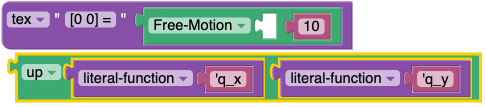
\includegraphics[scale=0.4]{bilder/session_51.png}
\caption{Der große Vorteil der graphischen Oberfläche: Ersetzen von Kacheln.}
\label{fig:session51}
\end{figure}

Die Funktion ''Path-of-a-Free-Particle'' kann jetzt aus der Benutzeroberfläche entfernt werden.
Der Ausgang dieses zweiten Computerexperiments ist sicherlich nicht jedem von vornherein klar, die Durchführung ist jedoch einfach, nämlich ein simpler Mausklick.

\begin{figure}[H]
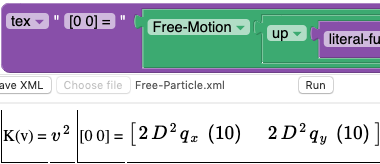
\includegraphics[scale=0.4]{bilder/session_62.png}
\caption{Das Ergebnis des zweiten Computerexperiments ist sicherlich erklärungsbedürftig.}
\label{fig:session62}
\end{figure}

Dieses Ergebnis ist überraschend und wird zum Staunen führen, es bedarf daher der genaueren Besprechung. Dem Wesen nach jedoch ist das Unverständnis vollkommen\todo{Eben nicht geklärt. Verbessern!} geklärt. Es besteht lediglich bezüglich der Interpretation der Formelzeichen des Ergebnisses. Denn die Rechenschritte werden von der Software durchgeführt, um deren Verständnis es zum Zeitpunkt des Experiments gar nicht geht\footnote{So geht es etwa auch einem Hochenergiephysiker bei Computersimulationen zur Effizienz eines bestimmten Zählrohrtypus nicht um das genaue Verständnis der nötigen Rechenschritte \cite{cKLMCern 21}.}.

Auch der Grund für die Verwendung einer unüblichen Notation wird rätselhaft sein, kann aber sofort geklärt werden. Der Vorteil dieser funktionalen Notation ist ihre sofortige Weiterverwendbarkeit, da sie leicht 1:1 in einen graphischen Block rückübersetzt werden könnte. In traditioneller Notation wird das Ergebnis wie folgt angeschrieben:

\begin{equation}
\begin{pmatrix} 0 \\ 0 \end{pmatrix} =
\begin{pmatrix} 
2 \frac{\mathrm d^2 x}{\mathrm d t^2} |_{t=10} \\ 
2 \frac{\mathrm d^2 y}{\mathrm d t^2} |_{t=10}
\end{pmatrix}
\end{equation}

Die genaue Besprechung folgt am besten \cite{cSussmanPaper 6} und wird beim Studierenden zum Verständnis der folgenden funktionalen Konzepte führen:

\begin{enumerate}[label=(\alph*)]
\item $q_x$ ist eine Funktion mit einer einzigen Variablen als Argument.
\item $D^2q_x$ ist die Bezeichnung für die zweite Ableitung dieser Funktion.
\item Es besteht kein Zweifel darüber, nach welcher Variablen abgeleitet wird. Im Ergebnis am Computer besitzt diese Variable jedoch keine Bezeichnung.
\item Im Speziellen kommt der Variablenname t am Computer nirgends vor.
\item Die zweite Ableitung einer Funktion ist wieder eine Funktion einer einzigen Variablen.
\end{enumerate}

Durch Hineinfügen einer die Masse repräsentierenden Kachel wird die kinetische Energie in die bekannte, allgemeine Form gebracht. Dieses immer wieder neue Hinzufügen und Weglöschen in der graphischen Oberfläche zeigt deutlich, dass hier ein verbessertes Modell aus einem vorhergehenden Modell entwickelt wird.

\begin{figure}[H]
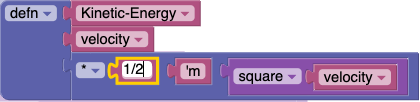
\includegraphics[scale=0.4]{bilder/session_70.png}
\caption{Verbesserung des Modelles durch Hinzufügen der Masse m zur in Abb. \ref{fig:session11} gezeigten kinetischen Energie.}
\label{fig:session70}
\end{figure}

Im letzten Schritt wird der Zeitpunkt 10 durch den Parameter t ersetzt, einem beliebig wählbaren, aber doch festen Zeitpunkt. Nachdem der Studierende das Experiment zum dritten Mal laufen lässt, sieht er am Bildschirm die Darstellung der Bewegungsgleichung \ref{eq:newton} des freien Teilchens.

\begin{figure}[H]
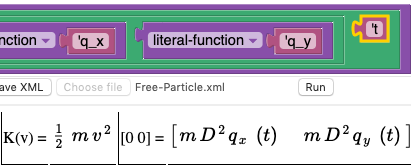
\includegraphics[scale=0.4]{bilder/session_82.png}
\caption{Das Endergebnis: Darstellung der Bewegungsgleichung des freien Teilchens \ref{eq:newton}.}
\label{fig:session82}
\end{figure}

Dieses Ergebnis sieht in üblicher Schreibweise etwas barock aus, weil die Unterscheidung zwischen Differentiationsvariable und Parameter zweier Buchstaben, $\tau$ und t, bedarf:

\begin{equation}
\begin{pmatrix} 0 \\ 0 \end{pmatrix} =
\begin{pmatrix} 
2 \frac{\mathrm d^2 x}{\mathrm d \tau^2} |_{\tau=t} \\ 
2 \frac{\mathrm d^2 y}{\mathrm d \tau^2} |_{\tau=t}
\end{pmatrix}
\end{equation}

Die am Beginn dieses Abschnitts dargestellte Gleichung

\begin{equation}
m \frac{\mathrm d^2 \vec{x}}{\mathrm d t^2}=0
\label{eq:newton2}
\end{equation}

ist dagegen einfacher und hier auch eindeutig. Oft erfolgt aber auch in komplizierten Fällen die Unterschlagung der zwischen Variable und Parameter dann so notwendigen Unterscheidung (siehe \cite{cSussmanPaper 6}). Ein Vorteil aller CAS ist, dass eine solche, wenn nötig, erzwungen wird. In funktionaler Notation ist diese in eleganter Weise immer gegeben.

\subsection{Zum Begriff Computerexperiment}
\todo{Sagt: das Gezeigte ist eben kein Experiment. Klingt widersprüchlich}Tatsache ist, dass das gerade gezeigte Computerprogramm zum freien Teilchen die Existenz des Teilchens selbst nicht erweisen kann. Daher wird an vielen Stellen argumentiert, dass keine Computersimulation ein Experiment sein kann. Dagegen vertritt \cite{cParker 22} (mit Referenzangaben) die Meinung, dass eine Simulation sehr wohl experimentellen Charakter haben kann, denn Tatsache ist auch, dass Computer gebaut und konfiguriert werden müssen.\todo{Computer eben auch ein physisches System ist. Aber nicht jedes p.S. ist ein Experiment.}

Wir vertreten hier folgenden Standpunkt: die Ansicht, dass unser Computerprogramm ein Experiment sei, ist zumindest eine notwendige Illusion. Und zwar in dem Sinne wie er von Gombrich in der Einleitung seiner Kunsttheorie vertreten wird \cite{cGombrich 23}: ''I, too, would stubbornly contend\todo{Was heisst contend? Übersetzen!} that I really see my head (natural size) when I shave and the $[ 50 \%]$ \todo{50\% wovon? Gesichts- Durchmesser auf Spiegel- oberfläche ist nur halb so groß wie reales Gesicht!} size on the mirror surface is the phantom. I cannot have my cake and eat it. I cannot make use of an illusion and watch it.'' 
Niemand kann in einem Portrait gleichzeitig die einzelnen Pinselstriche und das Gesamtbild gleichzeitig sehen. In diesem Sinne ist es besser, anstatt der einzelnen Computerbefehle das Experiment zu sehen. Ein Ziel der interaktiven Arbeit mit graphischen Bausteinen ist, diesen Sichtwechsel hervorzurufen. Denn diese Objekte lassen sich leicht mit echten Objekten identifizieren, allein schon wegen deren Bezeichnung als Kacheln und Blöcke.

Zur Motivation der didaktischen Sinnhaftigkeit des Begriffes ''Computerexperiment'' werden nun Zitate aus Krause \cite{cKrause 15} verwendet. Dies ist ein Artikel zur didaktischen Bedeutung realer Experimente, Computer spielen darin keine Rolle. Es ist bemerkenswert, wie gut diese Zitate in eine Betrachtung passen, in der die Studierenden das Computerprogramm als Experiment anerkennen.

Beispielsweise wäre so ein Computerexperiment ohne Theorie nicht denkbar. Und

''Demnach wäre es aus didaktischer Sicht sinnvoller, das Experiment den theoretischen Erwägungen anzuschließen.''

Die Abduktion ist ein ad hoc Schlussverfahren und wird wie folgt definiert:

''Ausgangspunkt einer Abduktion ist meist eine überraschende Tatsache, eine Frage oder eine Noch-Ungereimtheit, die eine Regel nahe legt, die die Frage beantwortet oder den Zweifel beseitigt. Das Staunen und Rätseln über empirische Phänomene sollte den kreativen Prozess des Begriffs- und Hypothesenbildens auslösen.''\todo{Die ganze Diskussion, was jetzt genau ein Experiemnt ist und was nicht ist ein weites Feld. Du meanderst drumrum, ohne wirklichen Mehrwert.}

Das zweite oben gezeigte Programmbeispiel führte zu einem Ergebnis mit vorerst unbekannter Notation, soll aber zum Verständnis des funktionalen Ansatzes führen. Je mehr der Dozent akzeptiert, dass dieses Ergebnis für den Studierenden ein empirisches Phänomen darstellen soll, desto naheliegender wird die Ansicht, dass im zweiten Beispiel dem Studenten beim Prozess des abduktiven Verstehens auf die Sprünge geholfen wird.

Damit das nächste Zitat verständlich wird, schlagen wir eine Beobachterposition vor, die eine Gruppe von Studierenden betrachtet. Der Beobachter sieht die Computer als reine Rechenmaschinen, währenddessen die Studierenden das erste oben gezeigte Computerexperiment zusammenbauen. Das Ergebnis (der Nullvektor) wird manchem Studierenden die physikalische Erkenntnis vermelden lassen, dass freie Teilchen tatsächlich geradeaus fliegen. Für den Beobachter gilt:
''Ausgehend von einem allgemeinen Prinzip ist durch einige mathematische Schritte eine neue physikalische Erkenntnis zutage gefördert worden.''

\subsection{Zusammenfassung und Ausblick}
In diesem Artikel wurde mithilfe einer graphischen Programmiersprache die Modellierung des einfachsten Falles der klassischen Mechanik vorgeführt, der Fall des freien Teilchens.  Der Vorteil der dafür ausgewählten funktionalen Notation zeigte sich beispielsweise in der klaren Unterscheidung zwischen Variable und Parameter. Das Einfügen von Funktionsansätzen in Differentialgleichungen war sehr schnell möglich, das Computerexperiment wurde dreimal adaptiert und laufengelassen. Dabei wurde durch die graphischen Möglichkeiten des Ersetzens von Programmteilen die graduelle Verbesserung des Modells anschaulich dargestellt und dadurch die Verwendung des Begriffs ''Computerexperiment'' für dieses interaktive Arbeiten nähergelegt. Daraus wird didaktisch besonders klar, dass Experimente theoriegebunden sind und dass rein theoretische Überlegungen zu physikalischen Erkenntnissen führen können.

Die dem System zugrundeliegende Programmbibliothek erlaubt die Modellierung von weiten Teilen der klassischen Mechanik. Tatsächlich wurden bereits viele weitere Beispiele in einem lauffähigen Notebook als Programmtext codiert \cite{cNextJ 24}. Die graphische Umsetzung dieser Beispiele sowie überhaupt ein Praxistest des Systems im Hörsaal stehen jedoch aus.

\begin{thebibliography}{999}
\bibitem {cSpencer 1}
Spencer, R. L. (2005): Teaching computational physics as a laboratory sequence. In: American journal of physics, Band 73, Nr. 2, S. 151-153.
\bibitem {cTimber 2}
Timberlake T. K.; Mixon, J. W. (2015): Classical Mechanics with Maxima, New York: Springer.
\bibitem {cRobi 3}
Robinett, R. W. (2007). Using Physics to Learn Mathematica to Do Physics: From Homework Problems to Research Examples. In: arXiv preprint arXiv:0712.2358.
\bibitem {cBerta 4}
Bertacchini, F.; Bilotta, E.; Caldarola, F.; Pantano, P. (2019): The role of computer simulations in learning analytic mechanics towards chaos theory: a course experimentation. In: International Journal of Mathematical Education in Science and Technology, Band 50, Nr. 1, S. 100-120.
\bibitem {cCaballero 5}
Caballero, M. D.; Merner, L. (2018): Prevalence and nature of computational instruction in undergraduate physics programs across the United States. In: Phys. Rev. Phys. Educ. Res., Band 14, Nr 2.
\bibitem {cSussmanPaper 6}
Sussman, G. J.; Wisdom, J. (2002): The Role of Programming in the Formulation of Ideas. \url{URL: ftp://publications.ai.mit.edu/ai-publications/2002/AIM-2002-018.pdf} (Stand: 19.8.2019)
\bibitem {cSICM 7}
Sussman, Gerald Jay; Wisdom, Jack (2014): Structure and Interpretation of Classical Mechanics, 2nd ed., Cambridge, MA: MIT Press. \url{URL: https://mitpress.mit.edu/sites/default/files/titles/content/sicm_edition_2/book.html} (Stand: 30.7.2019)
\bibitem {cDevelaki 8}
Develaki, M. (2019). Methodology and Epistemology of Computer Simulations and Implications for Science Education. In: Journal of Science Education and Technology, Band 28, Nr. 4, S. 1-18.
\bibitem {cBartPos 9}
Bart, A. C.; Tilevich, E.; Shaffer, C. A.; Kafura, D. (2015): Position paper: From interest to usefulness with BlockPy, a block-based, educational environment. In: 2015 IEEE Blocks and Beyond Workshop (Blocks and Beyond), S. 87-89.
\bibitem {cModrow 10}
Modrow, E. (2018): Informatik mit Snap. \url{URL: http://ddi-mod.uni-goettingen.de/InformatikMitSnap.pdf} (Stand: 30.7.2019)
\bibitem {cPrice 11}
Price, T. W.; Dong, Y.; Lipovac, D. (2017): iSnap: towards intelligent tutoring in novice programming environments. In: Proceedings of the 2017 ACM SIGCSE Technical Symposium on Computer Science Education, S. 483-488.

\bibitem {cXu 12}
Xu, Z.; Ritzhaupt, A. D.; Tian, F.; Umapathy, K. (2019): Block-based versus text-based programming environments on novice student learning outcomes: a metaanalysis study. In: Computer Science Education, Band 29, Nr. 2-3, S. 177-204.

\bibitem {cConversy 13}
Conversy, S. (2014): Unifying textual and visual: A theoretical account of the visual perception of programming languages. In: Proceedings of the 2014 ACM International Symposium on New Ideas, New Paradigms, and Reflections on Programming and Software, S. 201-212.

\bibitem {cLin 14}
Lin, S.; Aiken J. M.; Seaton D. T.; Douglas S. S.; Greco E. F.; Thomas B. D.; Schatz M. F. (2017): Exploring physics students’ engagement with online instructional videos in an introductory mechanics course. In: Phys. Rev. Phys. Educ. Res., Band 13, Nr. 2.
\bibitem {cKrause 15}
Krause, E. (2017): Einsteins EJASE-Modell als Ausgangspunkt physikdidaktischer Forschungsfragen. In: Physik und Didaktik in Schule und Hochschule, Band 1, Nr. 16. S. 57-66.
\bibitem {cScheme 16}
Abelson, H.; Sussman, G. J.; Sussman, J. (1996): Structure and Interpretation of Computer Programs, 2nd ed., Cambridge, MA: MIT Press. \url{URL: https://mitpress.mit.edu/sites/default/files/sicp/index.html} (Stand: 30.7.2019)
\bibitem {cMcCarthy 17}
McCarthy, J. (1960): Recursive functions of symbolic expressions and their computation by machine. In: Communications of the ACM, Band 3, Nr. 4, S. 184-195.
\bibitem {cColin 18}
Smith, C. (2019): Sicmutils in Clojure. \url{URL: https://github.com/littleredcomputer/sicmutils} (Stand: 30.7.2019)
\bibitem {cFraser 19}
Fraser, N. (2019): A JavaScript library for building visual programming editors. \url{URL: https://developers.google.com/blockly} (Stand: 30.7.2019)
\bibitem {cBartStudy 20}
Bart, A. C.; Tibau, J.; Kafura, D.; Shaffer, C. A.; Tilevich, E. (2017): Design and evaluation of a block-based environment with a data science context. In: IEEE Transactions on Emerging Topics in Computing.
\bibitem {cKLMCern 21}
XXXX (1998): CERN CMS-Note
\bibitem {cParker 22}
Parker, W. S. (2009): Does matter really matter? Computer simulations, experiments, and materiality. In: Synthese, Band 169, Nr. 3, S. 483-496.
\bibitem {cGombrich 23}
Gombrich, E. H. (1960): Art and Illusion, Princeton and Oxford: Princeton University Press
\bibitem {cNextJ 24}
XXXX (2019): \url{URL: https://nextjournal.com}
\end{thebibliography}

\end{document} 